\chapter{Positioning}\label{cha:position}

\section{Introduction}

This chapter discusses position, particularly how facets are laid out on
a page, and how coordinate systems within a panel work. There are four
components that control position. You have already learned about two of
them that work within a facet: \index{Positioning}

\begin{itemize}
\itemsep1pt\parskip0pt\parsep0pt
\item
  \textbf{Position adjustments} adjust the position of overlapping
  objects within a layer These are most useful for bar and other
  interval geoms, but can be useful in other situations
  (\hyperref[sec:position]{link to section}).
\item
  \textbf{Position scales} control how the values in the data are mapped
  to positions on the plot. Common transformations are linear and log,
  but any other invertible function can also be used
  (\hyperref[sub:scale-position]{link to section}).
\end{itemize}

This chapter will describe the other two components and show you how all
four components can be used together:

\begin{itemize}
\itemsep1pt\parskip0pt\parsep0pt
\item
  \textbf{Faceting} is a mechanism for automatically laying out multiple
  plots on a page. It splits the data into subsets, and then plots each
  subset into a different panel on the page. Such plots are often called
  small multiples (\hyperref[sec:faceting]{link to section}).
\item
  \textbf{Coordinate systems} control how the two independent position
  scales are combined to create a 2d coordinate system. The most common
  coordinate system is Cartesian, but other coordinate systems can be
  useful in special circumstances (\hyperref[sec:coord]{link to
  section}).
\end{itemize}

\hyperdef{}{sec:faceting}{\section{Faceting}\label{sec:faceting}}

You first encountered faceting in \hyperref[sec:qplot-faceting]{the
introduction to \texttt{qplot()}} and you may already have been using it
in your plots. Faceting generates small multiples each showing a
different subset of the data. Small multiples are a powerful tool for
exploratory data analysis: you can rapidly compare patterns in different
parts of the data and see whether they are the same or different. This
section will discuss how you can fine-tune facets, particularly the way
in which they interact with position scales. \index{Faceting}
\index{Positioning!faceting}

There are two types of faceting provided by \texttt{ggplot}:
\texttt{facet\_grid()} and \texttt{facet\_wrap()}. Facet grid produces a
2d grid of panels defined by variables which form the rows and columns,
while facet wrap produces a 1d ribbon of panels that is wrapped into 2d.
The grid layout is similar to the layout of \texttt{coplot} in base
graphics, and the wrapped layout is similar to the layout of panels in
\texttt{lattice}. These differences are illustrated in Figure
\ref{fig:facet-sketch}.

\begin{figure}[htbp]
  \centering
    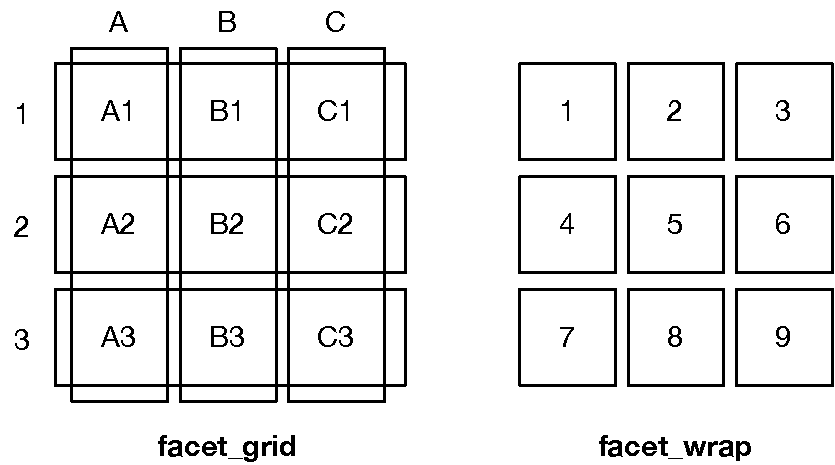
\includegraphics[width=0.5\linewidth]{diagrams/position-facets}
  \caption{A sketch illustrating the difference between the two faceting systems. \texttt{facet\_grid} (left) is fundamentally 2d, being made up of two independent components. \texttt{facet\_wrap} (right) is 1d, but wrapped into 2d to save space.}
  \label{fig:facet-sketch}
\end{figure}

There are two basic arguments to the faceting systems: the variables to
facet by, and whether position scales should be global or local to the
facet. The way these options are specified is a little different for the
two systems, so they are described separately below.

You can access either faceting system from \texttt{qplot()}. A 2d
faceting specification (e.g., \texttt{x \textasciitilde{} y}) will use
\texttt{facet\_grid()}, while a 1d specification (e.g.,
\texttt{\textasciitilde{} x}) will use \texttt{facet\_wrap()}.

Faceted plots have the capability to fill up a lot of space, so for this
chapter we will use a subset of the mpg dataset that has a manageable
number of levels: three cylinders (4, 6, 8) and two types of drive train
(4 and f). This removes 29 vehicles from the original dataset.

\begin{Shaded}
\begin{Highlighting}[]
\NormalTok{>}\StringTok{ }\NormalTok{mpg2 <-}\StringTok{ }\KeywordTok{subset}\NormalTok{(mpg, cyl !=}\StringTok{ }\DecValTok{5} \NormalTok{&}\StringTok{ }\NormalTok{drv %in%}\StringTok{ }\KeywordTok{c}\NormalTok{(}\StringTok{"4"}\NormalTok{, }\StringTok{"f"}\NormalTok{))}
\end{Highlighting}
\end{Shaded}

\subsection{Facet grid}

The grid faceter lays out plots in a 2d grid. When specifying a faceting
formula, you specify which variables should appear in the columns and
which should appear in the rows, as follows: \index{Faceting!grid}
\indexf{facet_grid}

\begin{itemize}
\item
  \texttt{. \textasciitilde{} .}: The default. Neither rows nor columns
  are faceted, so you get a single panel.

\begin{Shaded}
\begin{Highlighting}[]
\NormalTok{>}\StringTok{ }\KeywordTok{qplot}\NormalTok{(cty, hwy, }\DataTypeTok{data =} \NormalTok{mpg2) +}\StringTok{ }\KeywordTok{facet_null}\NormalTok{()}
\end{Highlighting}
\end{Shaded}

  \begin{flushleft}\includegraphics[width=0.49\linewidth]{figures/positionmpg2-null-1} \end{flushleft}
\item
  \texttt{. \textasciitilde{} a}: A single row with multiple columns.
  This is normally the most useful direction because computer screens
  are usually wider than they are long. This direction of faceting
  facilitates comparisons of y position, because the vertical scales are
  aligned.

\begin{Shaded}
\begin{Highlighting}[]
\NormalTok{>}\StringTok{ }\KeywordTok{qplot}\NormalTok{(cty, hwy, }\DataTypeTok{data =} \NormalTok{mpg2) +}\StringTok{ }\KeywordTok{facet_grid}\NormalTok{(. ~}\StringTok{ }\NormalTok{cyl)}
\end{Highlighting}
\end{Shaded}

  \begin{flushleft}\includegraphics[width=\linewidth]{figures/positionmpg2-grid-1} \end{flushleft}
\item
  \texttt{b \textasciitilde{} .}: A single column with multiple rows.
  This direction facilitates comparison of x position, because the
  horizontal scales are aligned, and so is particularly useful for
  comparing distributions. Figure \ref{fig:facet-hist} on page
  \pageref{fig:facet-hist} is a good example of this use.
\end{itemize}

\begin{Shaded}
\begin{Highlighting}[]
\NormalTok{>}\StringTok{ }\KeywordTok{qplot}\NormalTok{(cty, }\DataTypeTok{data =} \NormalTok{mpg2, }\DataTypeTok{geom=}\StringTok{"histogram"}\NormalTok{, }\DataTypeTok{binwidth =} \DecValTok{2}\NormalTok{) +}
\NormalTok{+}\StringTok{   }\KeywordTok{facet_grid}\NormalTok{(cyl ~}\StringTok{ }\NormalTok{.)}
\end{Highlighting}
\end{Shaded}

\begin{flushleft}\includegraphics[width=0.49\linewidth]{figures/positionmpg2-hist-1} \end{flushleft}

\begin{itemize}
\itemsep1pt\parskip0pt\parsep0pt
\item
  \texttt{a \textasciitilde{} b}: Multiple rows and columns. You'll
  usually want to put the variable with the greatest number of levels in
  the columns, to take advantage of the aspect ratio of your screen.
\end{itemize}

\begin{Shaded}
\begin{Highlighting}[]
\NormalTok{>}\StringTok{ }\KeywordTok{qplot}\NormalTok{(cty, hwy, }\DataTypeTok{data =} \NormalTok{mpg2) +}\StringTok{ }\KeywordTok{facet_grid}\NormalTok{(drv ~}\StringTok{ }\NormalTok{cyl)}
\end{Highlighting}
\end{Shaded}

\begin{flushleft}\includegraphics[width=\linewidth]{figures/positionmpg2-grid-both-1} \end{flushleft}

\begin{itemize}
\itemsep1pt\parskip0pt\parsep0pt
\item
  \texttt{. \textasciitilde{} a + b} or
  \texttt{a + b \textasciitilde{} .}: Multiple variables in the rows or
  columns (or both). This is unlikely to be useful unless the number of
  factor levels is small, you have a very wide screens or you want to
  produce a long, skinny poster.
\end{itemize}

Variables appearing together on the rows or columns are nested in the
sense that only combinations that appear in the data will appear in the
plot. Variables that are specified on rows and columns will be crossed:
all combinations will be shown, including those that didn't appear in
the original dataset: this may result in empty panels.

\subsubsection{Margins}\label{sub:margins}

Faceting a plot is like creating a contingency table. In contingency
tables it is often useful to display marginal totals (totals over a row
or column) as well as the individual cells. It is also useful to be able
to do this with graphics, and you can do so with the \texttt{margins}
argument. This allows you to compare the conditional patterns with the
marginal patterns. \index{Faceting!margins}

You can either specify that all margins should be displayed, using
\texttt{margins = TRUE}, or by listing the names of the variables that
you want margins for, \texttt{margins = c("sex", "age")}. You can also
use \texttt{"grand\_row"} or \texttt{"grand\_col"} to produce grand row
and grand column margins, respectively.

Figure \ref{fig:margins} shows what margins look like. The first plot
shows what the data looks like without margins, and the second shows all
margins. The margin column shows all drive trains, the margin row shows
all cylinders and the bottom right plot (the grand total) shows the full
dataset. For this data we can see that as the number of cylinders
increases, engine displacement increases and fuel economy decreases, and
compared to front-wheel-drive vehicles, as a group four-wheel-drive
vehicles have about the same displacement, but are less fuel efficient.
The figure was produced with the following code:

\begin{Shaded}
\begin{Highlighting}[]
\NormalTok{p <-}\StringTok{ }\KeywordTok{qplot}\NormalTok{(displ, hwy, }\DataTypeTok{data =} \NormalTok{mpg2) +}
\StringTok{  }\KeywordTok{geom_smooth}\NormalTok{(}\DataTypeTok{method =} \StringTok{"lm"}\NormalTok{, }\DataTypeTok{se =} \NormalTok{F)}
\NormalTok{p +}\StringTok{ }\KeywordTok{facet_grid}\NormalTok{(cyl ~}\StringTok{ }\NormalTok{drv) }
\NormalTok{p +}\StringTok{ }\KeywordTok{facet_grid}\NormalTok{(cyl ~}\StringTok{ }\NormalTok{drv, }\DataTypeTok{margins =} \NormalTok{T)}
\end{Highlighting}
\end{Shaded}

\begin{figure}

{\centering \includegraphics[width=0.49\linewidth]{figures/positionmargins-1} \includegraphics[width=0.49\linewidth]{figures/positionmargins-2} 

}

\caption{Graphical margins work like margins of a contingency table to give unconditioned views of the data.  A plot faceted by number of cylinders and drive train (left) is supplemented with margins (right).\label{fig:margins}}
\end{figure}

Groups in the margins are controlled in the same way as groups in all
other panels, defaulting to the interaction of all categorical variables
present in the layer. (See \hyperref[sub:grouping]{grouping} for a
reminder.) The following example shows what happens when we add a
coloured smooth for each drive train.

\begin{Shaded}
\begin{Highlighting}[]
\NormalTok{>}\StringTok{ }\KeywordTok{qplot}\NormalTok{(displ, hwy, }\DataTypeTok{data =} \NormalTok{mpg2) +}\StringTok{ }
\NormalTok{+}\StringTok{   }\KeywordTok{geom_smooth}\NormalTok{(}\KeywordTok{aes}\NormalTok{(}\DataTypeTok{colour =} \NormalTok{drv), }\DataTypeTok{method =} \StringTok{"lm"}\NormalTok{, }\DataTypeTok{se =} \NormalTok{F) +}\StringTok{ }
\NormalTok{+}\StringTok{   }\KeywordTok{facet_grid}\NormalTok{(cyl ~}\StringTok{ }\NormalTok{drv, }\DataTypeTok{margins =} \NormalTok{T) }
\end{Highlighting}
\end{Shaded}

\begin{flushleft}\includegraphics[width=0.49\linewidth]{figures/positionsmooths-1} \end{flushleft}

Plots with many facets and margins may be more appropriate for printing
than on screen display, as the higher resolution of print (600 dpi
vs.~72 dpi) allows you to compare many more subsets.

\subsection{Facet wrap}\label{sub:facet-wrap}

An alternative to the grid is a wrapped ribbon of plots. Instead of
having a 2d grid generated by the combination of two (or more)
variables, \texttt{facet\_wrap()} makes a long ribbon of panels
(generated by any number of variables) and wraps it into 2d. This is
useful if you have a single variable with many levels and want to
arrange the plots in a more space efficient manner. This is what
trellising in lattice does. \index{Faceting!wrapped} \indexf{facet_wrap}

Figure \ref{fig:movies-wrap} shows the distribution of average movie
ratings by decade. The main difference over time seems to be the
increasing spread of ratings. This is probably an artefact of the number
of votes: newer movies get more votes and so the average ratings are
likely to be less extreme. The disadvantage of this style of faceting is
that it is harder to compare some subsets that should be close together,
as in this example where the plots for the 50's and 60's are
particularly far apart because of the way the ribbon has been wrapped
around. The figure was produced with the following code:

\begin{Shaded}
\begin{Highlighting}[]
\NormalTok{movies$decade <-}\StringTok{ }\NormalTok{plyr::}\KeywordTok{round_any}\NormalTok{(movies$year, }\DecValTok{10}\NormalTok{, floor)}
\KeywordTok{qplot}\NormalTok{(rating, ..density.., }\DataTypeTok{data =} \KeywordTok{subset}\NormalTok{(movies, decade >}\StringTok{ }\DecValTok{1890}\NormalTok{),}
  \DataTypeTok{geom =} \StringTok{"histogram"}\NormalTok{, }\DataTypeTok{binwidth =} \FloatTok{0.5}\NormalTok{) +}\StringTok{ }
\StringTok{  }\KeywordTok{facet_wrap}\NormalTok{(~}\StringTok{ }\NormalTok{decade, }\DataTypeTok{ncol =} \DecValTok{6}\NormalTok{)}
\end{Highlighting}
\end{Shaded}

\begin{figure}

{\centering \includegraphics[width=\linewidth]{figures/positionmovies-wrap-1} 

}

\caption{Movie rating distribution by decade.\label{fig:movies-wrap}}
\end{figure}

The specification of faceting variables is of the form
\texttt{\textasciitilde{} a + b + c}. By default, \texttt{facet\_wrap()}
will try and lay out the panels as close to a square as possible, with a
slight bias towards wider rather than taller rectangles. You can
override the default by setting \texttt{ncol}, \texttt{nrow} or both.
See the documentation for more examples.

\subsection{Controlling scales}\label{sub:controlling-scales}

For both types of faceting you can control whether the position scales
are the same in all panels (fixed) or allowed to vary between panels
(free). This is controlled by the \texttt{scales} parameter:
\index{Faceting!interaction with scales}
\index{Scales!interaction with facetting}
\index{Faceting!controlling scales}

\begin{itemize}
\itemsep1pt\parskip0pt\parsep0pt
\item
  \texttt{scales = "fixed"}: x and y scales are fixed across all panels.
\item
  \texttt{scales = "free"}: x and y scales vary across panels.
\item
  \texttt{scales = "free\_x"}: the x scale is free, and the y scale is
  fixed.
\item
  \texttt{scales = "free\_y"}: the y scale is free, and the x scale is
  fixed.
\end{itemize}

Figure \ref{fig:fixed-vs-free} illustrates the difference between the
two extremes of fixed and free.

\begin{Shaded}
\begin{Highlighting}[]
\NormalTok{p <-}\StringTok{ }\KeywordTok{qplot}\NormalTok{(cty, hwy, }\DataTypeTok{data =} \NormalTok{mpg)}
\NormalTok{p +}\StringTok{ }\KeywordTok{facet_wrap}\NormalTok{(~}\StringTok{ }\NormalTok{cyl)}
\NormalTok{p +}\StringTok{ }\KeywordTok{facet_wrap}\NormalTok{(~}\StringTok{ }\NormalTok{cyl, }\DataTypeTok{scales =} \StringTok{"free"}\NormalTok{)}
\end{Highlighting}
\end{Shaded}

\begin{figure}

{\centering \includegraphics[width=0.49\linewidth]{figures/positionfixed-vs-free-1} \includegraphics[width=0.49\linewidth]{figures/positionfixed-vs-free-2} 

}

\caption{Fixed scales (left) have the same scale for each facet, while free scales (right) have a different scale for each facet. \label{fig:fixed-vs-free}}
\end{figure}

Fixed scales allow us to compare subsets on an equal basis, seeing where
each fits into the overall pattern. Free scales zoom in on the region
that each subset occupies, allowing you to see more details. Free scales
are particularly useful when we want to display multiple times series
that were measured on different scales. To do this, we first need to
change from `wide' to `long' data, stacking the separate variables into
a single column. An example of this is shown in Figure \ref{fig:time},
and the topic is discussed in more detail in
\hyperref[sec:melting]{converting data from wide to long}.

\begin{Shaded}
\begin{Highlighting}[]
\NormalTok{em <-}\StringTok{  }\NormalTok{tidyr::}\KeywordTok{gather}\NormalTok{(economics, variable, value, -date)}
\KeywordTok{qplot}\NormalTok{(date, value, }\DataTypeTok{data =} \NormalTok{em, }\DataTypeTok{geom =} \StringTok{"line"}\NormalTok{, }\DataTypeTok{group =} \NormalTok{variable) +}\StringTok{ }
\StringTok{  }\KeywordTok{facet_grid}\NormalTok{(variable ~}\StringTok{ }\NormalTok{., }\DataTypeTok{scale =} \StringTok{"free_y"}\NormalTok{)}
\end{Highlighting}
\end{Shaded}

\begin{figure}

{\centering \includegraphics[width=\linewidth]{figures/positiontime-1} 

}

\caption{Free scales are particularly useful when displaying multiple time series measured on different scales.\label{fig:time}}
\end{figure}

There is an additional constraint on the scales of
\texttt{facet\_grid()}: all panels in a column must have the same x
scale, and all panels in a row must have the same y scale. This is
because each column shares an x axis, and each row shares a y axis.

For \texttt{facet\_grid()} there is an additional parameter called
\texttt{space}, which takes values \texttt{"free"} or \texttt{"fixed"}.
When the space can vary freely, each column (or row) will have width (or
height) proportional to the range of the scale for that column (or row).
This makes the scaling equal across the whole plot: 1 cm on each panel
maps to the same range of data. (This is somewhat analogous to the
`sliced' axis limits of lattice.) For example, if panel a had range 2
and panel b had range 4, one-third of the space would be given to a, and
two-thirds to b. This is most useful for categorical scales, where we
can assign space proportionally based on the number of levels in each
facet, as illustrated by Figure \ref{fig:discrete-free}. The code to
create this plot is shown below: note the use of \texttt{reorder()} to
arrange the models and manufacturers in order of city fuel usage.
\index{Faceting!panel size}

\begin{Shaded}
\begin{Highlighting}[]
\NormalTok{mpg3 <-}\StringTok{ }\KeywordTok{within}\NormalTok{(mpg2, \{}
  \NormalTok{model <-}\StringTok{ }\KeywordTok{reorder}\NormalTok{(model, cty)}
  \NormalTok{manufacturer <-}\StringTok{ }\KeywordTok{reorder}\NormalTok{(manufacturer, -cty)}
\NormalTok{\})}
\NormalTok{models <-}\StringTok{ }\KeywordTok{qplot}\NormalTok{(cty, model, }\DataTypeTok{data =} \NormalTok{mpg3)}

\NormalTok{models}
\NormalTok{models +}\StringTok{ }\KeywordTok{facet_grid}\NormalTok{(manufacturer ~}\StringTok{ }\NormalTok{., }\DataTypeTok{scales =} \StringTok{"free"}\NormalTok{, }
  \DataTypeTok{space =} \StringTok{"free"}\NormalTok{) +}\StringTok{ }\KeywordTok{theme}\NormalTok{(}\DataTypeTok{strip.text.y =} \KeywordTok{element_text}\NormalTok{(}\DataTypeTok{angle =} \DecValTok{0}\NormalTok{))}
\end{Highlighting}
\end{Shaded}

\begin{figure}

{\centering \includegraphics[width=0.49\linewidth]{figures/positiondiscrete-free-1} \includegraphics[width=0.49\linewidth]{figures/positiondiscrete-free-2} 

}

\caption{A dotplot showing the range of city gas mileage for each model of car. (Left) Models ordered by average mpg, and (right) faceted by manufacturer with \texttt{scales='free\_y'} and \texttt{space = 'free'}. The \texttt{strip.text.y} theme setting has been used to rotate the facet labels.\label{fig:discrete-free}}
\end{figure}

\subsection{Missing faceting
variables}\label{sub:missing-faceting-columns}

If you are using faceting on a plot with multiple datasets, what happens
when one of those datasets is missing the faceting variables? This
situation commonly arises when you are adding contextual information
that should be the same in all panels. For example, imagine you have a
spatial display of disease faceted by gender. What happens when you add
a map layer that does not contain the gender variable? Here ggplot will
do what you expect: it will display the map in every facet: missing
faceting variables are treated like they have all values.
\index{Faceting!missing data}

\subsection{Grouping vs.~faceting}\label{sub:group-vs-facet}

Faceting is an alternative to using aesthetics (like colour, shape or
size) to differentiate groups. Both techniques have strengths and
weaknesses, based around the relative positions of the subsets.
\index{Faceting!vs. grouping} \index{Grouping!vs. faceting}

With faceting, each group is quite far apart in its own panel, and there
is no overlap between the groups. This is good if the groups overlap a
lot, but it does make small differences harder to see. When using
aesthetics to differentiate groups, the groups are close together and
may overlap, but small differences are easier to see. Figure
\ref{fig:group-vs-facet} illustrates these trade-offs. With the
scatterplots, it is possible to not realise the groups are overlapping
when just colour is used to separate them, but with the regression lines
they are too far apart to see that D, E and G are grouped together and J
is farther away. The code to produce these figures is shown below.

\begin{Shaded}
\begin{Highlighting}[]
\NormalTok{xmaj <-}\StringTok{ }\KeywordTok{c}\NormalTok{(}\FloatTok{0.3}\NormalTok{, }\FloatTok{0.5}\NormalTok{, }\DecValTok{1}\NormalTok{,}\DecValTok{3}\NormalTok{, }\DecValTok{5}\NormalTok{)}
\NormalTok{xmin <-}\StringTok{ }\KeywordTok{as.vector}\NormalTok{(}\KeywordTok{outer}\NormalTok{(}\DecValTok{1}\NormalTok{:}\DecValTok{10}\NormalTok{, }\DecValTok{10}\NormalTok{^}\KeywordTok{c}\NormalTok{(-}\DecValTok{1}\NormalTok{, }\DecValTok{0}\NormalTok{)))}
\NormalTok{ymaj <-}\StringTok{ }\KeywordTok{c}\NormalTok{(}\DecValTok{500}\NormalTok{, }\DecValTok{1000}\NormalTok{, }\DecValTok{5000}\NormalTok{, }\DecValTok{10000}\NormalTok{)}
\NormalTok{ymin <-}\StringTok{ }\KeywordTok{as.vector}\NormalTok{(}\KeywordTok{outer}\NormalTok{(}\DecValTok{1}\NormalTok{:}\DecValTok{10}\NormalTok{, }\DecValTok{10}\NormalTok{^}\KeywordTok{c}\NormalTok{(}\DecValTok{2}\NormalTok{,}\DecValTok{3}\NormalTok{,}\DecValTok{4}\NormalTok{)))}
\NormalTok{dplot <-}\StringTok{ }\KeywordTok{ggplot}\NormalTok{(}\KeywordTok{subset}\NormalTok{(diamonds, color %in%}\StringTok{ }\KeywordTok{c}\NormalTok{(}\StringTok{"D"}\NormalTok{,}\StringTok{"E"}\NormalTok{,}\StringTok{"G"}\NormalTok{,}\StringTok{"J"}\NormalTok{)), }
  \KeywordTok{aes}\NormalTok{(carat, price, }\DataTypeTok{colour =} \NormalTok{color)) +}\StringTok{ }
\StringTok{  }\KeywordTok{scale_x_log10}\NormalTok{(}\DataTypeTok{breaks =} \NormalTok{xmaj, }\DataTypeTok{labels =} \NormalTok{xmaj, }\DataTypeTok{minor =} \NormalTok{xmin) +}\StringTok{ }
\StringTok{  }\KeywordTok{scale_y_log10}\NormalTok{(}\DataTypeTok{breaks =} \NormalTok{ymaj, }\DataTypeTok{labels =} \NormalTok{ymaj, }\DataTypeTok{minor =} \NormalTok{ymin) +}\StringTok{ }
\StringTok{  }\KeywordTok{scale_colour_hue}\NormalTok{(}\DataTypeTok{limits =} \KeywordTok{levels}\NormalTok{(diamonds$color)) +}\StringTok{ }
\StringTok{  }\KeywordTok{theme}\NormalTok{(}\DataTypeTok{legend.position =} \StringTok{"none"}\NormalTok{)}

\NormalTok{dplot +}\StringTok{ }\KeywordTok{geom_point}\NormalTok{()}
\NormalTok{dplot +}\StringTok{ }\KeywordTok{geom_point}\NormalTok{() +}\StringTok{ }\KeywordTok{facet_grid}\NormalTok{(. ~}\StringTok{ }\NormalTok{color)}

\NormalTok{dplot +}\StringTok{ }\KeywordTok{geom_smooth}\NormalTok{(}\DataTypeTok{method =} \NormalTok{lm, }\DataTypeTok{se =} \NormalTok{F, }\DataTypeTok{fullrange =} \NormalTok{T)}
\NormalTok{dplot +}\StringTok{ }\KeywordTok{geom_smooth}\NormalTok{(}\DataTypeTok{method =} \NormalTok{lm, }\DataTypeTok{se =} \NormalTok{F, }\DataTypeTok{fullrange =} \NormalTok{T) +}\StringTok{ }
\StringTok{  }\KeywordTok{facet_grid}\NormalTok{(. ~}\StringTok{ }\NormalTok{color)}
\end{Highlighting}
\end{Shaded}

\begin{figure}

{\centering \includegraphics[width=0.49\linewidth]{figures/positiongroup-vs-facet-1} \includegraphics[width=0.49\linewidth]{figures/positiongroup-vs-facet-2} \includegraphics[width=0.49\linewidth]{figures/positiongroup-vs-facet-3} \includegraphics[width=0.49\linewidth]{figures/positiongroup-vs-facet-4} 

}

\caption{The differences between faceting vs. grouping, illustrated with a log-log plot of carat vs. price with four selected colours.\label{fig:group-vs-facet}}
\end{figure}

Faceting will also work with a much larger number of groups, and because
you can split in two dimensions, you can compare two variables
simultaneously more easily than using two different aesthetics. The
other advantage of faceting is that the scales can vary across panels,
which is useful if the subsets occupy very different ranges.

\subsection{Dodging vs.~faceting}\label{sub:dodge-vs-facet}

Faceting can achieve similar effects to dodging. Figure
\ref{fig:fvd-crossed} shows how dodging and faceting can create plots
that look remarkably similar. The main difference is the labelling: the
faceted plot has colour labelled above and cut below; and the dodged
plot has colour below and cut is not explicitly labelled. In this
example, the labels in the faceted plot need some adjustment to display
in a readable way, see the code below for details.
\index{Dodging!vs. faceting} \index{Faceting!vs. dodging}
\indexf{geom_bar}

\begin{Shaded}
\begin{Highlighting}[]
\KeywordTok{qplot}\NormalTok{(color, }\DataTypeTok{data =} \NormalTok{diamonds, }\DataTypeTok{geom =} \StringTok{"bar"}\NormalTok{, }\DataTypeTok{fill =} \NormalTok{cut, }
  \DataTypeTok{position =} \StringTok{"dodge"}\NormalTok{)}
\KeywordTok{qplot}\NormalTok{(cut, }\DataTypeTok{data =} \NormalTok{diamonds, }\DataTypeTok{geom =} \StringTok{"bar"}\NormalTok{, }\DataTypeTok{fill =} \NormalTok{cut) +}\StringTok{ }
\StringTok{  }\KeywordTok{facet_grid}\NormalTok{(. ~}\StringTok{ }\NormalTok{color) +}\StringTok{ }
\StringTok{  }\KeywordTok{theme}\NormalTok{(}\DataTypeTok{axis.text.x =} \KeywordTok{element_text}\NormalTok{(}\DataTypeTok{angle =} \DecValTok{90}\NormalTok{, }\DataTypeTok{hjust =} \DecValTok{1}\NormalTok{, }\DataTypeTok{size =} \DecValTok{8}\NormalTok{, }
   \DataTypeTok{colour =} \StringTok{"grey50"}\NormalTok{))}
\end{Highlighting}
\end{Shaded}

\begin{figure}

{\centering \includegraphics[width=0.8\linewidth]{figures/positionfvd-crossed-1} \includegraphics[width=0.8\linewidth]{figures/positionfvd-crossed-2} 

}

\caption{Dodging (top) vs. faceting (bottom) for a completely crossed pair of variables.\label{fig:fvd-crossed}}
\end{figure}

Apart from labelling, the main difference between dodging and faceting
occurs when the two variables are nearly completely crossed, but there
are some combinations that do not occur. In this case, dodging becomes
less useful because it only splits up the bars locally, and there are no
labels. Faceting is more useful as we can control whether the splitting
is local (\texttt{scales = "free\_x"}, \texttt{space = "free"}) or
global (\texttt{scales = "fixed"}). Figure \ref{fig:fvd-nested} compares
faceting and dodging for two nested variables from the \texttt{mpg}
dataset, model and manufacturer, with the code shown below.

\begin{Shaded}
\begin{Highlighting}[]
\NormalTok{mpg4 <-}\StringTok{ }\KeywordTok{subset}\NormalTok{(mpg, manufacturer %in%}\StringTok{ }
\StringTok{  }\KeywordTok{c}\NormalTok{(}\StringTok{"audi"}\NormalTok{, }\StringTok{"volkswagen"}\NormalTok{, }\StringTok{"jeep"}\NormalTok{))}
\NormalTok{mpg4$manufacturer <-}\StringTok{ }\KeywordTok{as.character}\NormalTok{(mpg4$manufacturer)}
\NormalTok{mpg4$model <-}\StringTok{ }\KeywordTok{as.character}\NormalTok{(mpg4$model)}

\NormalTok{base <-}\StringTok{ }\KeywordTok{ggplot}\NormalTok{(mpg4, }\KeywordTok{aes}\NormalTok{(}\DataTypeTok{fill =} \NormalTok{model)) +}\StringTok{ }
\StringTok{  }\KeywordTok{geom_bar}\NormalTok{(}\DataTypeTok{position =} \StringTok{"dodge"}\NormalTok{) +}\StringTok{ }
\StringTok{  }\KeywordTok{theme}\NormalTok{(}\DataTypeTok{legend.position =} \StringTok{"none"}\NormalTok{)}

\NormalTok{base +}\StringTok{ }\KeywordTok{aes}\NormalTok{(}\DataTypeTok{x =} \NormalTok{model) +}\StringTok{ }
\StringTok{  }\KeywordTok{facet_grid}\NormalTok{(. ~}\StringTok{ }\NormalTok{manufacturer)}
  
\KeywordTok{last_plot}\NormalTok{() +}\StringTok{  }
\StringTok{  }\KeywordTok{facet_grid}\NormalTok{(. ~}\StringTok{ }\NormalTok{manufacturer, }\DataTypeTok{scales =} \StringTok{"free_x"}\NormalTok{, }\DataTypeTok{space =} \StringTok{"free"}\NormalTok{)}
\NormalTok{base +}\StringTok{ }\KeywordTok{aes}\NormalTok{(}\DataTypeTok{x =} \NormalTok{manufacturer)}
\end{Highlighting}
\end{Shaded}

\begin{figure}

{\centering \includegraphics[width=0.8\linewidth]{figures/positionfvd-nested-1} \includegraphics[width=0.8\linewidth]{figures/positionfvd-nested-2} \includegraphics[width=0.8\linewidth]{figures/positionfvd-nested-3} 

}

\caption{For nested data, there is a clear advantage to faceting (top and middle) compared to dodging (bottom), because it is possible to carefully control and label the facets.  For this example, the top plot is not useful, but it will be useful in situations where the data is almost crossed, i.e. where a single combination is missing.\label{fig:fvd-nested}}
\end{figure}

In summary, the choice between faceting and dodging depends on the
relationship between the two variables:

\begin{itemize}
\itemsep1pt\parskip0pt\parsep0pt
\item
  Completely crossed: faceting and dodging are basically equivalent.
\item
  Almost crossed: faceting with shared scales ensures that all
  combinations are visible, even if empty. This is particularly useful
  if missing combinations are non-structural missings.
\item
  Nested: faceting with free scales and space allocates just enough
  space for each higher level group, and labels each item individually.
\end{itemize}

\subsection{Continuous variables}\label{sub:continuous-variables}

You can facet by continuous variables, but you will need to convert them
into discrete categories first. There are three ways to do this:
\index{Faceting!by continuous variables}

\begin{itemize}
\itemsep1pt\parskip0pt\parsep0pt
\item
  Divide the data into n bins each of the same length:
  \texttt{cut\_interval(x, n = 10)} to specify the number of bins, or
  \texttt{cut\_interval(x, length = 1)} to specify the length of each
  interval. Specifying the number of bins is easy, but may produce
  ranges that are not ``nice'' numbers. \indexf{cut_interval}
\item
  Divide the data into n bins each containing (approximately) the same
  number of points: \texttt{cut\_number(x, n = 10)}. This makes it
  easier to compare facets (they will all have the same number of
  points), but you need to note that the range of each bin is different.
  \indexf{cut_number}
\end{itemize}

The following code demonstrates each of the three possibilities, with
the results shown in Figure \ref{fig:discretising}.

\begin{Shaded}
\begin{Highlighting}[]
\NormalTok{mpg2$disp_ww <-}\StringTok{ }\KeywordTok{cut_interval}\NormalTok{(mpg2$displ, }\DataTypeTok{length =} \DecValTok{1}\NormalTok{)}
\NormalTok{mpg2$disp_wn <-}\StringTok{ }\KeywordTok{cut_interval}\NormalTok{(mpg2$displ, }\DataTypeTok{n =} \DecValTok{6}\NormalTok{)}
\NormalTok{mpg2$disp_nn <-}\StringTok{ }\KeywordTok{cut_number}\NormalTok{(mpg2$displ, }\DataTypeTok{n =} \DecValTok{6}\NormalTok{)}

\NormalTok{plot <-}\StringTok{ }\KeywordTok{qplot}\NormalTok{(cty, hwy, }\DataTypeTok{data =} \NormalTok{mpg2) +}\StringTok{ }\KeywordTok{labs}\NormalTok{(}\DataTypeTok{x =} \OtherTok{NULL}\NormalTok{, }\DataTypeTok{y =} \OtherTok{NULL}\NormalTok{)}
\NormalTok{plot +}\StringTok{ }\KeywordTok{facet_wrap}\NormalTok{(~}\StringTok{ }\NormalTok{disp_ww, }\DataTypeTok{nrow =} \DecValTok{1}\NormalTok{)}
\NormalTok{plot +}\StringTok{ }\KeywordTok{facet_wrap}\NormalTok{(~}\StringTok{ }\NormalTok{disp_wn, }\DataTypeTok{nrow =} \DecValTok{1}\NormalTok{)}
\NormalTok{plot +}\StringTok{ }\KeywordTok{facet_wrap}\NormalTok{(~}\StringTok{ }\NormalTok{disp_nn, }\DataTypeTok{nrow =} \DecValTok{1}\NormalTok{)}
\end{Highlighting}
\end{Shaded}

\begin{figure}

{\centering \includegraphics[width=0.9\linewidth]{figures/positiondiscretising-1} \includegraphics[width=0.9\linewidth]{figures/positiondiscretising-2} \includegraphics[width=0.9\linewidth]{figures/positiondiscretising-3} 

}

\caption{ Three ways of breaking a continuous variable into discrete bins. From top to bottom: bins of length one, six bins of equal length, six bins containing equal numbers of points.\label{fig:discretising}}
\end{figure}

Note that the faceting formula only works with variables in the dataset
(not functions of the variables), so you will also need to create a new
variable containing the discretised data.

\hyperdef{}{sec:coord}{\section{Coordinate systems}\label{sec:coord}}

Coordinate systems tie together the two position scales to produce a 2d
location. Currently, \texttt{ggplot} comes with six different coordinate
systems, listed in Table \ref{tbl:coord}. All these coordinate systems
are two dimensional, although one day I hope to add 3d graphics too. As
with the other components in \texttt{ggplot}, you generate the R name by
joining \texttt{coord\_} and the name of the coordinate system. Most
plots use the default Cartesian coordinate system,
\texttt{coord\_cartesian()}, where the 2d position of an element is
given by the combination of the x and y positions.
\index{Coordinate systems} \index{Positioning!coordinate systems}

Coordinate systems have two main jobs:

\begin{itemize}
\itemsep1pt\parskip0pt\parsep0pt
\item
  Combine the two position aesthetics to produce a 2d position on the
  plot. The position aesthetics are called \texttt{x} and \texttt{y},
  but they might be better called position 1 and 2 because their meaning
  depends on the coordinate system used. For example, with the polar
  coordinate system they become angle and radius (or radius and angle),
  and with maps they become latitude and longitude.
\item
  In coordination with the faceter, coordinate systems draw axes and
  panel backgrounds. While the scales control the values that appear on
  the axes, and how they map from data to position, it is the coordinate
  system which actually draws them. This is because their appearance
  depends on the coordinate system: an angle axis looks quite different
  than an x axis.
\end{itemize}

\subsection{Transformation}\label{sub:coord-transformation}

Unlike transforming the data or transforming the scales, transformations
carried out by the coordinate system change the appearance of the geoms:
in polar coordinates a rectangle becomes a slice of a doughnut; in a map
projection, the shortest path between two points will no longer be a
straight line. Figure \ref{fig:coord-trans-examples} illustrates what
happens to a line and a rectangle in a few different coordinate systems.
\index{Transformation!coordinate system}

\begin{figure}

{\centering \includegraphics[width=0.25\linewidth]{figures/positioncoord-trans-examples-1} \includegraphics[width=0.25\linewidth]{figures/positioncoord-trans-examples-2} \includegraphics[width=0.25\linewidth]{figures/positioncoord-trans-examples-3} \includegraphics[width=0.25\linewidth]{figures/positioncoord-trans-examples-4} \includegraphics[width=0.25\linewidth]{figures/positioncoord-trans-examples-5} \includegraphics[width=0.25\linewidth]{figures/positioncoord-trans-examples-6} 

}

\caption{A set of examples illustrating what a line and rectangle look like when displayed in a variety of coordinate systems.  From top left to bottom right: Cartesian, polar with x position mapped to angle, polar with y position mapped to angle, flipped, transformed with log in y direction, and equal scales.\label{fig:coord-trans-examples}}
\end{figure}

This transformation takes part in two steps. Firstly, the
parameterisation of each geom is changed to be purely location-based,
rather than location and dimension based. For example, a bar can be
represented as an x position (a location), a height and a width (two
dimensions). But how do we interpret height and width in a non-Cartesian
coordinate system, where a rectangle may not have constant height and
width? We solve the problem by using a purely location-based
representation, the location of the four corners of the rectangle, and
then transforming these locations: we have converted a rectangle to a
polygon. By doing this, we effectively convert all geoms to a
combination of points, lines and polygons.
\index{Geoms!parameterisation} \index{Coordinate systems!transformation}

With all geoms in this consistent, location-based, representation, the
next step is to transform each location into the new coordinate system.
It is easy to transform points, because a point is still a point no
matter what coordinate system you are in, but lines and polygons are
harder, because a straight line may no longer be straight in the new
coordinate system. To make the problem tractable we assume that all
coordinate transformations are smooth, in the sense that all very short
lines will still be very short straight lines in the new coordinate
system. With this assumption in hand, we can transform lines and
polygons by breaking them up into many small line segments and
transforming each segment. This process is called munching.
\index{Munching} Figure \ref{fig:coord-trans} illustrates this
procedure. We start with a line parameterised by its two endpoints, then
break it into multiple line segments, each with two endpoints. Those
points are then translated into the new coordinate system, and
connected. In the example, the number of line segments is too small, so
you can see more easily how it works. For practical use, we use many
more segments so that the result looks smooth.

\begin{figure}

{\centering \includegraphics[width=0.32\linewidth]{figures/positioncoord-trans-1} \includegraphics[width=0.32\linewidth]{figures/positioncoord-trans-2} \includegraphics[width=0.32\linewidth]{figures/positioncoord-trans-3} \includegraphics[width=0.32\linewidth]{figures/positioncoord-trans-4} \includegraphics[width=0.32\linewidth]{figures/positioncoord-trans-5} \includegraphics[width=0.32\linewidth]{figures/positioncoord-trans-6} 

}

\caption{How coordinate transformations work: converting a line in Cartesian coordinates to a line in polar coordinates.  The original x position is converted to radius, and the y position to angle.\label{fig:coord-trans}}
\end{figure}

\subsection{Statistics}\label{sub:statistics}

To be technically correct, the actual statistical method used by a stat
should depend on the coordinate system. For example, a smoother in polar
coordinates should use circular regression, and in 3d should return a 2d
surface rather than a 1d curve. However, many statistical operations
have not been derived for non-Cartesian coordinates and \texttt{ggplot}
falls back to Cartesian coordinates for calculation, which, while not
strictly correct, will normally be a fairly close approximation.
\index{Coordinate systems!interaction with scales}
\index{Scales!interaction with coordinate system}

\subsection{Cartesian coordinate systems}\label{sub:cartesian}

The four Cartesian-based coordinate systems,
\texttt{coord\_cartesian()}, \texttt{coord\_equal()},
\texttt{coord\_flip()} and \texttt{coord\_trans()}, share a number of
common features. They are still essentially Cartesian because the x and
y positions map orthogonally to x and y positions on the plot.
\index{Coordinate systems!Cartesian} \indexf{coord_cartesian}

\textbf{Setting limits.}

\texttt{coord\_cartesian()} has arguments \texttt{xlim} and
\texttt{ylim}. If you think back to the scales chapter, you might wonder
why we need these. Doesn't the limits argument of the scales already
allow us to control what appears on the plot? The key difference is how
the limits work: when setting scale limits, any data outside the limits
is thrown away; but when setting coordinate system limits we still use
all the data, but we only display a small region of the plot. Setting
coordinate system limits is like looking at the plot under a magnifying
glass. Figures\textasciitilde{}\ref{fig:limits-smooth}
and\textasciitilde{}\ref{fig:limits-bin} show an example of this.
\index{Zooming} \index{Axis!limits}

\begin{Shaded}
\begin{Highlighting}[]
\NormalTok{(p <-}\StringTok{ }\KeywordTok{qplot}\NormalTok{(disp, wt, }\DataTypeTok{data=}\NormalTok{mtcars) +}\StringTok{ }\KeywordTok{geom_smooth}\NormalTok{())}
\NormalTok{p +}\StringTok{ }\KeywordTok{scale_x_continuous}\NormalTok{(}\DataTypeTok{limits =} \KeywordTok{c}\NormalTok{(}\DecValTok{325}\NormalTok{, }\DecValTok{500}\NormalTok{))}
\NormalTok{p +}\StringTok{ }\KeywordTok{coord_cartesian}\NormalTok{(}\DataTypeTok{xlim =} \KeywordTok{c}\NormalTok{(}\DecValTok{325}\NormalTok{, }\DecValTok{500}\NormalTok{))}
\end{Highlighting}
\end{Shaded}

\begin{figure}

{\centering \includegraphics[width=0.32\linewidth]{figures/positionlimits-smooth-1} \includegraphics[width=0.32\linewidth]{figures/positionlimits-smooth-2} \includegraphics[width=0.32\linewidth]{figures/positionlimits-smooth-3} 

}

\caption{Setting limits on the coordinate system, vs setting limits on the scales.  (Left) Entire dataset; (middle) x scale limits set to (325, 500); (right) coordinate system x limits set to (325, 500).  Scaling the coordinate limits performs a visual zoom, while setting the scale limits subsets the data and refits the smooth.\label{fig:limits-smooth}}
\end{figure}

\begin{Shaded}
\begin{Highlighting}[]
\NormalTok{(d <-}\StringTok{ }\KeywordTok{ggplot}\NormalTok{(diamonds, }\KeywordTok{aes}\NormalTok{(carat, price)) +}\StringTok{ }
\StringTok{  }\KeywordTok{stat_bin2d}\NormalTok{(}\DataTypeTok{bins =} \DecValTok{25}\NormalTok{, }\DataTypeTok{colour=}\StringTok{"grey70"}\NormalTok{) +}\StringTok{ }
\StringTok{  }\KeywordTok{theme}\NormalTok{(}\DataTypeTok{legend.position =} \StringTok{"none"}\NormalTok{)) }
\NormalTok{d +}\StringTok{ }\KeywordTok{scale_x_continuous}\NormalTok{(}\DataTypeTok{limits =} \KeywordTok{c}\NormalTok{(}\DecValTok{0}\NormalTok{, }\DecValTok{2}\NormalTok{))}
\NormalTok{d +}\StringTok{ }\KeywordTok{coord_cartesian}\NormalTok{(}\DataTypeTok{xlim =} \KeywordTok{c}\NormalTok{(}\DecValTok{0}\NormalTok{, }\DecValTok{2}\NormalTok{))}
\end{Highlighting}
\end{Shaded}

\begin{figure}

{\centering \includegraphics[width=0.32\linewidth]{figures/positionlimits-bin-1} \includegraphics[width=0.32\linewidth]{figures/positionlimits-bin-2} \includegraphics[width=0.32\linewidth]{figures/positionlimits-bin-3} 

}

\caption{Setting limits on the coordinate system, vs. setting limits on the scales.  (Left) Entire dataset; (middle) x scale limits set to (0, 2); (right) coordinate x limits set to (0, 2).  Compare the size of the bins: when you set the scale limits, there are the same number of bins but they each cover a smaller region of the data; when you set the coordinate limits, there are fewer bins and they cover the same amount of data as the original.\label{fig:limits-bin}}
\end{figure}

\textbf{Flipping the axes.}

Most statistics and geoms assume you are interested in y values
conditional on x values (e.g., smooth, summary, boxplot, line): in most
statistical models, the x values are assumed to be measured without
error. If you are interested in x conditional on y (or you just want to
rotate the plot 90 degrees), you can use \texttt{coord\_flip()} to
exchange the x and y axes. Compare this with just exchanging the
variables mapped to x and y, as shown in Figure \ref{fig:coord-flip}.
\index{Rotating} \index{Coordinate systems!flipping the axes}
\indexf{coord_flip}

\begin{Shaded}
\begin{Highlighting}[]
\KeywordTok{qplot}\NormalTok{(displ, cty, }\DataTypeTok{data =} \NormalTok{mpg) +}\StringTok{ }\KeywordTok{geom_smooth}\NormalTok{()}
\KeywordTok{qplot}\NormalTok{(cty, displ, }\DataTypeTok{data =} \NormalTok{mpg) +}\StringTok{ }\KeywordTok{geom_smooth}\NormalTok{()}
\KeywordTok{qplot}\NormalTok{(cty, displ, }\DataTypeTok{data =} \NormalTok{mpg) +}\StringTok{ }\KeywordTok{geom_smooth}\NormalTok{() +}\StringTok{ }\KeywordTok{coord_flip}\NormalTok{()}
\end{Highlighting}
\end{Shaded}

\begin{figure}

{\centering \includegraphics[width=0.32\linewidth]{figures/positioncoord-flip-1} \includegraphics[width=0.32\linewidth]{figures/positioncoord-flip-2} \includegraphics[width=0.32\linewidth]{figures/positioncoord-flip-3} 

}

\caption{(Left) A scatterplot and smoother with engine displacement on x axis and city mpg on y axis.  (Middle) Exchanging \texttt{cty} and \texttt{displ} rotates the plot 90 degrees, but the smooth is fit to the rotated data.  (Right) using \texttt{coord\_flip()} fits the smooth to the original data, and then rotates the output, this is a smooth curve of x conditional on y.\label{fig:coord-flip}}
\end{figure}

\textbf{Transformations.}

Like limits, we can also transform the data in two places: at the scale
level or at the coordinate system level. \texttt{coord\_trans()} has
arguments \texttt{x} and \texttt{y} which should be strings naming the
transformer (Table \ref{tbl:common-trans}) to use for that axis.
Transforming at the scale level occurs before statistics are computed
and does not change the shape of the geom. Transforming at the
coordinate system level occurs after the statistics have been computed,
and does affect the shape of the geom. Using both together allows us to
model the data on a transformed scale and then backtransform it for
interpretation: a common pattern in analysis. An example of this is
shown in Figure \ref{fig:backtrans}.
\index{Transformation!coordinate system}
\index{Coordinate systems!transformation} \indexf{coord_trans}

\begin{Shaded}
\begin{Highlighting}[]
\NormalTok{pow10 <-}\StringTok{ }\NormalTok{scales::}\KeywordTok{exp_trans}\NormalTok{(}\DecValTok{10}\NormalTok{)}
\KeywordTok{qplot}\NormalTok{(carat, price, }\DataTypeTok{data =} \NormalTok{diamonds, }\DataTypeTok{log =} \StringTok{"xy"}\NormalTok{) +}\StringTok{ }
\StringTok{  }\KeywordTok{geom_smooth}\NormalTok{(}\DataTypeTok{method =} \StringTok{"lm"}\NormalTok{)}
\KeywordTok{last_plot}\NormalTok{() +}\StringTok{ }\KeywordTok{coord_trans}\NormalTok{(}\DataTypeTok{x =} \NormalTok{pow10, }\DataTypeTok{y =} \NormalTok{pow10)}
\end{Highlighting}
\end{Shaded}

\begin{figure}

{\centering \includegraphics[width=0.49\linewidth]{figures/positionbacktrans-1} \includegraphics[width=0.49\linewidth]{figures/positionbacktrans-2} 

}

\caption{(Left) A scatterplot of carat vs. price on log base 10 transformed scales.  A linear regression summarises the trend: $\log(y) = a + b * \log(x)$.  (Right) The previous plot backtransformed (with \texttt{coord\_trans(x = 'pow10', y = 'pow10')}) onto the original scales.  The linear trend line now becomes geometric, $y = k * c^x$, and highlights the lack of expensive diamonds for larger carats.\label{fig:backtrans}}
\end{figure}

\textbf{Equal scales.}

\texttt{coord\_equal()} ensures that the x and y axes have equal scales:
i.e., 1 cm along the x axis represents the same range of data as 1 cm
along the y axis. By default it will assume that you want a one-to-one
ratio, but you can change this with the \texttt{ratio} parameter. The
aspect ratio will also be set to ensure that the mapping is maintained
regardless of the shape of the output device. See the documentation of
\texttt{coord\_equal()} for more details. \index{Aspect ratio}
\index{Coordinate systems!Equal scales} \indexf{coord_equal}

\subsection{Non-Cartesian coordinate systems}

There are two non-Cartesian coordinate systems: polar coordinates and
map projections. These coordinate systems are still somewhat
experimental, and there are fewer standards for the layout of axes, so
you may need to tweak them to meet your needs using the tools in
\hyperref[cha:grid]{grid}. \index{Coordinate systems!non-Cartesian}

\textbf{Polar coordinates.}

Using polar coordinates gives rise to pie charts and wind roses (from
bar geoms), and radar charts (from line geoms). Polar coordinates are
often used for circular data, particularly time or direction, but the
perceptual properties are not good because the angle is harder to
perceive for small radii than it is for large radii. The \texttt{theta}
argument determines which position variable is mapped to angle (by
default, x) and which to radius. Figure \ref{fig:polar} shows how by
changing the coordinate system we can turn a bar chart into a pie chart
or a bullseye chart. The documentation includes other examples of polar
charts. \index{Polar coordinates} \index{Coordinate systems!polar}
\indexf{coord_polar}

\begin{Shaded}
\begin{Highlighting}[]
\CommentTok{# Stacked barchart}
\NormalTok{(pie <-}\StringTok{ }\KeywordTok{ggplot}\NormalTok{(mtcars, }\KeywordTok{aes}\NormalTok{(}\DataTypeTok{x =} \KeywordTok{factor}\NormalTok{(}\DecValTok{1}\NormalTok{), }\DataTypeTok{fill =} \KeywordTok{factor}\NormalTok{(cyl))) +}
\StringTok{  }\KeywordTok{geom_bar}\NormalTok{(}\DataTypeTok{width =} \DecValTok{1}\NormalTok{))}
\CommentTok{# Pie chart}
\NormalTok{pie +}\StringTok{ }\KeywordTok{coord_polar}\NormalTok{(}\DataTypeTok{theta =} \StringTok{"y"}\NormalTok{)}

\CommentTok{# The bullseye chart}
\NormalTok{pie +}\StringTok{ }\KeywordTok{coord_polar}\NormalTok{()}
\end{Highlighting}
\end{Shaded}

\begin{figure}

{\centering \includegraphics[width=0.32\linewidth]{figures/positionpolar-1} \includegraphics[width=0.32\linewidth]{figures/positionpolar-2} \includegraphics[width=0.32\linewidth]{figures/positionpolar-3} 

}

\caption{(Left) A stacked bar chart.  (Middle) The stacked bar chart in polar coordinates, with x position mapped to radius and y position mapped to angle, \texttt{coord\_polar(theta = 'y')}).  This is more commonly known as a pie chart.  (Right) The stacked bar chart in polar coordinates with the opposite mapping, \texttt{coord\_polar(theta = 'x')}. This is sometimes called a bullseye chart.\label{fig:polar}}
\end{figure}

\textbf{Map projections.}

These are still rather experimental, and rely on the \textbf{mapproj}
package (McIlroy 2005). \texttt{coord\_map()} takes the same arguments
as \texttt{mapproj()} for controlling the projection. See the
documentation of \texttt{coord\_map()} for more examples, and consult a
cartographer for the most appropriate projection for your data.
\index{Maps!projections} \index{Coordinate systems!map projections}
\indexf{coord_map}

McIlroy, Doug. 2005. \emph{Mapproj: Map Projections}.
